\documentclass[conference]{IEEEconf}
%\documentclass[sigconf]{acmart}
\usepackage{cite}
\usepackage{amsmath,amssymb,amsfonts}
\usepackage{algorithmic}
\usepackage{graphicx}
\usepackage{textcomp}
\usepackage{xcolor}
\usepackage{url}
%\usepackage{hyperref}
%\usepackage{latex8}
%\usepackage{times}
%\pagestyle{empty}
%\usepackage{epsfig}
%\def\BibTeX{{\rm B\kern-.05em{\sc i\kern-.025em b}\kern-.08em
%    T\kern-.1667em\lower.7ex\hbox{E}\kern-.125emX}}
    
\bibliographystyle{IEEEtran}
\graphicspath{./images/}

\newcommand{\mq}{\mbox{\em MQ}}

\title{ 
        	Cloud Native Software Engineering 
      }


\author{
			Brian Mitchell\\
			College of Computing and Informatics\\
			Drexel University, Philadelphia, PA, USA\\
			bmitchell@drexel.edu
} 

\date{}

\begin{document}

%\bibliographystyle{latex8}

\maketitle

\thispagestyle{empty}


\begin{abstract}

The adoption of cloud computing has been growing in popularity since its inception in the early 2000's with all signs pointing to continued growth over the remainder of the decade\cite{IDCReport}. While there is a significant research activity in many areas of cloud computing, we see little attention being paid to advancing software engineering practices needed to support the next generation of cloud native applications.  By cloud native, we mean software that is designed and built specifically for deployment to a modern cloud platform. This paper will focus on the landscape of Cloud Native Software Engineering from a practitioners standpoint, and  identify opportunities that we think should be investigated by the software engineering research community.

\end{abstract}  



\section{Introduction and Context}
\label{Intro}
Delivering managed computing services via hosted infrastructure stared in the late 1990's with the introduction of the Software as a Service (SaaS) model. One of the early pioneers of this model is Salesforce.com, launched in 1999\cite{SalesforceHistory}.  Unlike other companies that licensed software that deployed to on premise equipment, Salesforce provides a pay-as-you-go SaaS subscription model. In this model, they manage all of the software and compute, you pay a monthly per-user charge that can access the solution from any device at any time.     

While SaaS solutions marked the start of shifting software license spend to usage-based spend, cloud computing as we know it today can be attributed to the launch of AWS (Amazon) \cite{AWSLaunch} in early 2006, with Azure (Microsoft)\cite{AzureLaunch} and GCP (Google)\cite{GCPLaunch} following in 2008. The primary early adopters of cloud computing were technology companies that innovated patterns, practices, and open sourced many tools and frameworks that have become best practices for running resilient and scalable business services in the public cloud.  It's probably been less than 10 years, but now we see acceptance of cloud computing in companies of all sizes across many different industries. 

Larry Wall, the creator of Perl, is credited with a quote that has become a popular software engineering meme -- \textit{"Good. Fast. Cheap. Pick two."}.  There is some intuitive merit to this insight given software engineering is a rooted in making informed tradeoffs.  For example, it would not be hard to argue that in order to move faster and build things cheaper, you will need to compromise on software features and/or software quality. Using the utility of the cloud, coupled with modern cloud computing tooling, one can now argue that you can build better software faster and cheaper.  It's not that Larry Wall's insights were incorrect, but we can now have the technologies and practices to redefine \textit{good} in terms of \textit{fast} using the cloud.  When computing components are deployed to the cloud, the simplest way (and thus the most popular way) to do this is via automation technologies\cite{terraform, AWSCloudFormation, AzureLaunch, Pulumi}.  The \textit{automate everything} practice embraced by cloud computing not only allows deployments to be fast, but it also favors ephemeral computing components. These components by their nature are easier to test\cite{kim2016devops} and can be started, stopped, paused, or replaced at any time. 

This combination of capabilities enables software engineers to rapidly deploy software to a known state at any time. With these building blocks new well-tested features can be quickly and consistently rolled out to users in very small batches.  Goodness of the solution can now be validated via feedback from users, either directly, or via monitoring and instrumentation of their behavior.  These cloud enabled capabilities have the potential to advanced software engineering practices in many ways, but transforming these practices across the entire community will be challenging. We think this represents a significant opportunity for the software engineering field given the likelihood that most industrial systems moving forward will be deployed on cloud runtimes\footnote{By cloud runtime we include public, private and hybrid cloud infrastructure}. Specifically:

\begin{enumerate}
	\item \vspace{-0.2cm}Helping Software Engineers manage the expanded cognitive required to design, build and deploy at scale cloud applications. We will discuss this throughout the remaining sections of this paper. 
	
	\item \vspace{-0.2cm}Identify opportunities to accelerate and scale software engineering skillsets needed to deploy a broader suite of applications the cloud. Many industries will strive to move beyond deploying externally facing web and mobile applications to the cloud using their top engineers. This will require developing new skills for the broader engineering organization as more of their core business processing moves to the cloud.
	
	\item \vspace{-0.2cm}Investigate how software engineering and computer science education can expand to address the demands of industry to create new, and retooling existing software engineers for the cloud.\footnote{We will talk about cloud certifications later, but they are targeted towards using the services of a cloud provider, not designing cloud native applications} Most cloud-proficient software engineers build their skillsets on the job versus in formalized academic programs. 
	
	\item \vspace{-0.2cm}Understand software engineering needs for new architectures enabled by the cloud.  For example, IoT and smart devices that run at the edge increase the complexity of software engineering given the increasing distributed nature of these solutions.  These challenges will be discussed in a later section of this paper
\end{enumerate}

In the next section we start by providing a definition for cloud native computing. Subsequent sections will build on trends in cloud native computing that we think will impact software engineering practices.  Throughout this paper, by cloud native, we are referring to systems designed specifically to favor managed cloud platform services (PaaS/Faas)\cite{albuquerque2017function}, and not systems that are \textit{lifted and shifted}\cite{CloudMigration2017} from an on premise virtual machine to a virtual machine that runs in the cloud (IaaS). 


\section{What is Cloud Native Computing?}
\label{sec:WhatIsCNF}


Before we explore the software engineering landscape for the cloud, we need to address exactly what we mean by cloud native computing.  According to the Cloud Native Computing Foundation (CNCF)\cite{CNCFHome}  \textit{"Cloud native technologies empower organizations to build and run scalable applications in modern, dynamic environments such as public, private, and hybrid clouds."}.  Amazon's definition is \textit{"Cloud native technologies empower organizations to build and run scalable applications in modern, dynamic environments such as public, private, and hybrid clouds"}. Google offers the definition \textit{"Cloud native means adapting to the many new possibilities—but very different set of architectural constraints—offered by the cloud compared to traditional on-premises infrastructure."}.  The primary theme in these definitions centers around the role that technologies play in enabling the creation of cloud native applications.  They also don't clearly define "Cloud Native", which we consider any application that is specifically designed to be deployed to a cloud platform. 

We think a better definition of cloud native computing that focuses more on  software engineering is \textit{"Cloud native applications are well architected systems, that are "container" packaged, and dynamically managed"}. Specifically:

\begin{figure*}[t]
	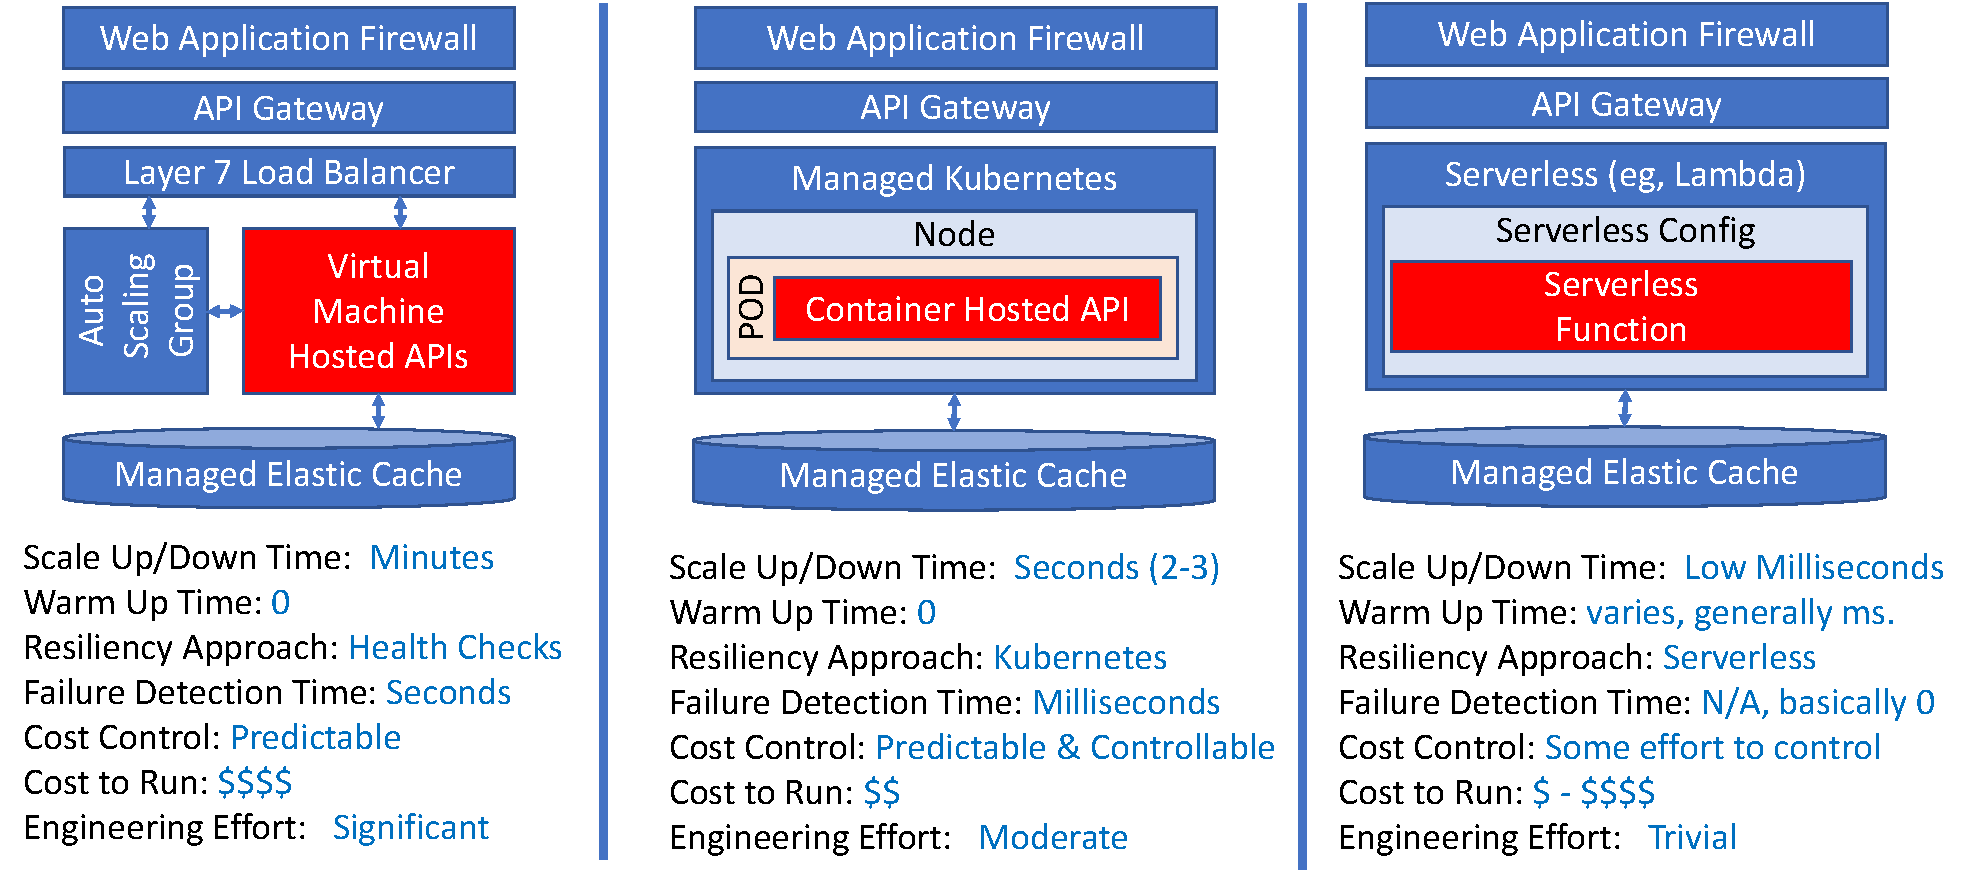
\includegraphics[width=\textwidth]{images/APIPackageTradoffs}	
	\caption{Cloud Native Architectural Tradeoffs for a Hypothetical Suite of APIs}
	\label{fig:CloudQATradeoffs}
\end{figure*}

\textbf{Well Architected Systems} - By this we mean systems that adhere not only to established software engineering best practices but also embrace specific functional and non-functional capabilities offered by the cloud. For example, how are the computing components identified, how are they work with each other, how are security requirements met, how is the system designed for resiliency and scale?

\textbf{Container Packaged} - The term \textit{container} is overloaded in the cloud computing terminology landscape.  In many places its equated to a standardized package that is managed by Docker\cite{DockerContainer} technologies - aka "a docker container".  We take a more generic view of container packaging. Specifically, we think container packaging is a mechanism to package and deploy code that is ephemeral, can operate across a variety of different hardware architectures (e.g., Intel, ARM, etc), and at runtime is supervised.  Supervision includes full lifecycle management associated with version identification, startup, shutdown, health checks, and monitoring.  Examples of container packaging and supervision include Docker, Docker Compose, Kubernetes, and serverless \cite{baldini2017serverless}. We also include in this category the emerging popularity of using server-side web assembly\cite{haas2017bringing, bosshard2020use} as a way to package and deploy cloud native application services. 

\textbf{Dynamically Managed} - One interesting conceptual model for cloud computing is to consider the cloud as a large, highly distributed, special purpose operating system. Just like any operating system, there are a number of resource like storage, compute, network and security services that are needed by applications.  The job of an operating system is to dynamically manage and optimize the allocation of these resources to the realtime computing demand on the system.  When done well, every process being managed by the OS will perceive that it has access to the resources it needs, when it needs it.  In a similar context, a cloud service provider, via Application Programming Interfaces (APIs), provides and manages resources to cloud native applications dynamically. What is generally different is that an OS manages physical resources on a system, whereas cloud resources are generally virtualized and distributed, and to a large degree fault-tolerant.  For example, block storage that supports virtual machine reads and writes are automatically replicated across servers within an availability zone. Outside of initial configuration, the user does not worry about how durability is provided given its dynamically managed by the cloud service provider. Other examples include using auto scaling of virtual machines with health checks, or more advanced services like kubernetes\cite{kubernetes} that can scale up or down dynamically based on demand. Function as a service (FaaS) solution's take this a step further by configuring what code should be run when a certain event happens.     

Now that we have provided a definition, we describe next a number of interesting software engineering problems that warrant investigation.

\textit{Managing cloud native technical assets}.  In 2011 Adam Wiggins authored a set of technical principals that enable software engineers to create, manage and release code in support of cloud native applications. These principals were branded "The Twelve-Factor App"\cite{12factor}.  Over the years they were updated and revalidated\cite{hoffman2016beyond, 12factorRevisited}, but consistently hold up as recommended engineering practices. One of the key challenges is that while none of these practices is overly complex, they require mastery and discipline. Also, existing standards enforced by enterprises might act as blockers to some or all of these practices.  For example, some organizations might not have comfort or necessary controls to ensure that all deploys, to all environments are driven through the source code control system.

\textit{Identifying an appropriate cloud native software architecture}.  The technical principals associated with 12 factor apps is a good start, however, these only focus on how to manage cloud native technical assets.  Good cloud native architectures are generally architected as a suite of horizontally composable components. This model introduces several interesting challenges for cloud native software engineers that must be addressed. What are these components? How do identify them? What will guide how they should be built? We think some of the newer concepts around app meshes\cite{GartnerMASA} and data meshes\cite{datamesh} provide a good start for shaping the overall architecture.  As far as identifying the architecture components themselves, we think concepts from Domain Driven Design (DDD)\cite{evans2004domain, vernon2013implementing} can be refreshed to support this activity.

\textit{Upskilling Software Engineers on the use Quality Attributes to make informed technology tradeoff decisions}. Most cloud providers offer many different technology choices to create cloud native components.  Applying discipline around the desired quality attributes should guide making technology stack decisions. For example, Figure\ref{fig:CloudQATradeoffs} shows three different ways to deploy cloud native APIs along with some quality attributes.  It should be noted, that the values of these quality attributes will change for different APIs, the figure assumes these hypothetical APIs are very light weight, event triggered, and manage their state via a clustered cache.  Thus for the scenario shown in the figure, the VM option does not make a lot of sense given the high cost, large scale up/down times, and complex engineering effort.  The container option in the middle and the serverless option on the right both seem like good options.  The ultimate decision will be driven by the desire to have a high degree of control over cost, and the nature of the workload. For example, if the expected traffic has massive near realtime spikes, a serverless solution might be preferred. If the workload is not event-driven, or has many runtime dependencies such as database connections, then a container based solution might be a better choice. As we move more towards computing at the edge, containers might not be possible since they depend on Linux, so emerging lighter weight alternatives such as WebAssembly with WASI\cite{WASI} might be a good choice.  Cloud native software engineers must be able to make these types of choices and resist over-standardizing based on personal or organizational preference on the best runtime for a cloud native component. 

\textit{Organizing teams for cloud native success}.  In 1967, Mel Conway published a paper called "How Do Committees Invent" - Fred Brooks cited this paper in the Mythical Man Month\cite{Brooks1975} calling it Conways law\cite{ConwaysLaw}. Conways law states \textit{"Any organization that designs a system (defined broadly) will produce a design whose structure is a copy of the organization's communication structure"}.  In the early days of Amazon, Jeff Bazos introduced the idea of the "2 pizza team rule"\cite{TwoPizza} where a team size should be no larger than can be fed by two pizzas.  The basic ideas are rooted in concepts that productive teams should be small, and independent.  This aligns nicely with cloud native concepts in that one way to ensure that components are independent and interoperate only via their published interfaces, that teams are also organized this way.  Over the years various organizational models and changes have been debated. \textit{Full-stack teams} bring together front-end, back-end, testing and infrastructure professionals to a common team where they have full responsibility over their technical assets. \textit{Shifting left} along with the emergence of \textit{DevOps} brings a testing and automation focus to teams that allows them to increase productivity.  One problem is that while these concepts work well for driving individual team productivity, they are difficult to scale to larger organizations.  Several companies have also published their attempts to scale their practices.  One popular model was published by Spotify\cite{SpotifyModel}, where "Squads" represent full-stack teams, but they also introduce concepts like "Tribes" for coordinating squads, and "Guilds" to address cross-cutting technical concerns. Commercial models have also been created to drive organizational changes to support cloud native architectures.  One such example is the SAFe\cite{SAFeAgile} framework, which is interesting in that it favors prescriptive organization and process rigor over streamlining software engineering practices in order to increase scale. We think there are some interesting problems in this space given the lack of alignment on the best ways to organize teams to work on cloud native applications at scale. Specifically, just copying a model used in one organization and using it in another organization does not address many of the challenges associated with things like politics and culture. 

\begin{figure}
	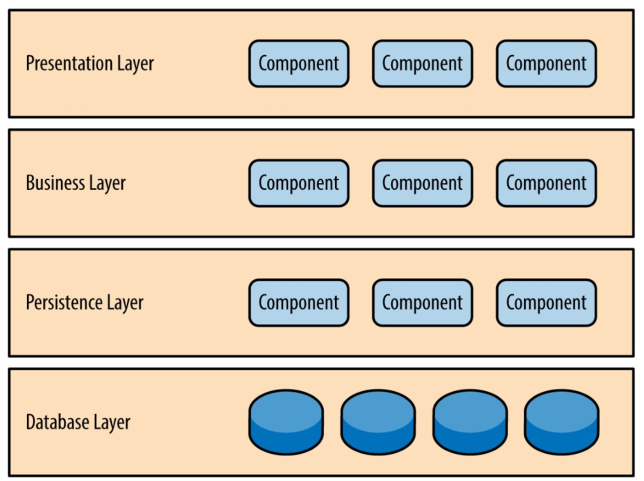
\includegraphics[width=\columnwidth]{images/LayeredArchitecture}	
	\caption{Layered Software Architecture}
	\label{fig:LayeredArchitecture}
\end{figure}

\textit{Software engineering demands for API based technical products}.  Historically, most applications are built to solve a targeted user or business problem end-to-end.  In Mark Richards book entitled "Software Architecture Patterns"\cite{richards2015software}, Chapter 1 is focused on the \textit{Layered Architecture Pattern}, which is shown in Figure \ref{fig:LayeredArchitecture}. Richards shows this pattern containing 4 layers, but other variations exist like the 3-tier architecture that just focus on the presentation, business logic, and database layers are widely used. We found references going back to 1996\cite{aarsten1996patterns} describing this pattern. One of the foundational enablers of cloud computing is the plethora of first-class integration services provided by the platform. These capabilities open the door for new software architectures based on offering API-enabled services as a product. Several well known examples of this new type of product are Google Maps (for location services), Twilio (for messaging), and Stripe (for payment). These all represent API-based products designed to be OEMd into other applications. All signs point to this business model expanding and will require software engineers to become familiar with designing API-centric products.  For example, some of the best AI models are offered as a service by OpenAI\cite{OpenAI}, and the healthcare industry is being mandated to offer API services to support interoperability\cite{FHIRAPI} regulations.  Some of these companies are even taking the opportunities to use APIs as a competitive differentiator, one example is the developer portal provided by Cigna\cite{CignaDeveloper}. Prior to the mainstream adoption of the cloud it would be unusual to think that you could work with your bank, healthcare provider, auto insurer, and favorite retail stores via developing software. 


\begin{figure*}[t!]
	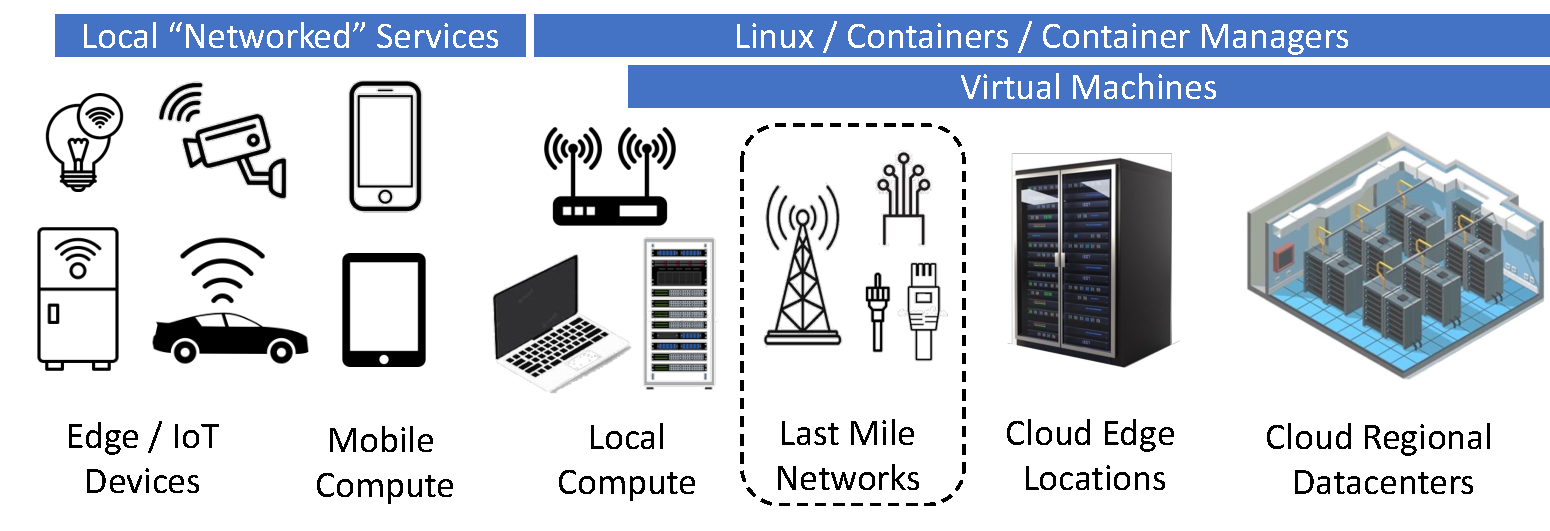
\includegraphics[width=\textwidth]{images/CloudTopo2.pdf}	
	\caption{The Modern Cloud}
	\label{fig:CloudTopo}
\end{figure*}

\section{The Cloud is Expanding to the Edge}
\label{sec:CloudArchitecture}



The underlying services that the major cloud providers offer to their customers continues to expand and evolve.  These advancements provide significant innovation capabilities to customers, but also put pressure on how to effectively engineer solutions that take advantage of these services cost effectively.  Figure \ref{fig:CloudTopo} shows the high level view of the modern cloud.  While it was once easy to identify the boundary of where the cloud started and ended, it is no longer easy to define the edge of the cloud.  The following sections will provide an overview of the evolution of the cloud, along with highlighting some of the challenges that have to be overcome by software engineers to effectively use cloud computing services in their products.

\subsection{The Basic Cloud Architecture}

At a high level the basic cloud architectures deployed by major providers exhibit many similarities\footnote{It should be noted that the terminology used by the major cloud providers differs slightly for things like availability zones and regions.}.  The foundational infrastructure building block of cloud compute is called an \textbf{Availability Zone} (AZ).  An AZ is a data center that hosts cloud infrastructure (compute, storage, and network) and runs cloud provider services on behalf of their customers.  A \textbf{Region} is a physical location where a collection of 2 or more AZs are located.  Each AZ within a region are connected together with a fully redundant high bandwidth low latency network.  The goal of a region is to have AZs close enough so that they can behave like a single cluster, but also separate them by enough distance to isolate them from issues associated with power failure, earthquakes, tornados, and so on.  AWS, as an example, uses the general guideline of 100km (60 miles)\cite{AWS-AZ} for placing AZs within a region. The global footprint of a cloud provider is defined by the number of regions and locations they have across the globe, along with the purpose-built underlying network they use to interconnect them together. 

Given the cost and complexity of deploying cloud regions around the globe, cloud providers expand their network reach through the use of edge locations.  Edge locations are useful for a couple of reasons. First, they serve as a point of presence to lower connection latency to the cloud, and second, they can run services at the edge which offers additional benefits.  One of the classical applications to run at the edge is a content delivery network (CDN). CDNs speed up web and mobile applications. For digital web and mobile applications the combination of Regions, AZs, and Edge Locations could be considered the boundary of the cloud. These are shown on the right side of Figure\ref{fig:CloudTopo}.      

From a software engineering perspective, the basic cloud architecture described above introduces additional cognitive load on software engineers:

\begin{itemize}
	\item \vspace{-0.2cm} Planning application deployment starts with the design of a virtual data center (VDC). VDCs logically carve out storage, compute, network and security policies from the cloud provider for customer usage. Traditional software engineers are not trained to think of the start of the software design process begins with the need to design a virtual data center and all of the complexity that comes with it.  Historically, data centers are designed by specialty engineers and inherited "as is" into the final software architecture. The data center topology is now a critical software engineering concern. 
	
	\item \vspace{-0.2cm} Quality attributes such as privacy, resiliency, reliability and scalability are foundational concepts that software architects use to reason about systems.  These now move out of the conceptual realm and require a deeper understanding of technical constructs that now become part of the software design itself.  For example, deploying microservices across different subnets, where each subnet is in a different AZ within a region. Also, declarative definition of  the security policies that govern access to these microservices along with their entitlements to access other cloud resources becomes part of the software product itself. 
	
	\item \vspace{-0.2cm} Although the cloud itself provides an infrastructure model to create resilient solutions that run at scale, its up to the software engineer to architect things properly to take advantage of these capabilities\footnote{Some patterns such as rehosting\cite{engelsrud2019moving} {\em a.k.a.} "lift-and-shift" should not be considered cloud native patterns.}.  For example, it's still possible to deploy an application to a single virtual machine instance in the cloud, which will not elastically scale, nor will it be resilient to failure.  Thus, to enable the creation of cloud services software engineers must have mastery of newer patterns for distributed applications ( {\em e.g.}, especially asynchronous event-based architectures).
	
	\item \vspace{-0.2cm} While cybersecurity has always been an important consideration of software engineers, the cloud materially expands these responsibilities. Everything in the cloud is secured by policy, but as mentioned earlier, software engineers now need to deal with security requirements across the entire OSI model\cite{OSIModel} stack in addition to some unique cloud requirements. Generally software engineers are comfortable with security at Layer 7 (the Application Layer) of the OSI model, using techniques such as OAuth 2\cite{oAuthStandard} to secure different types of digital assets. These responsibilities now expand to authoring and deploying policies to govern network access across subnets, and for attaching policies necessary to use managed services.  In addition, software engineers must deploy and ensure proper configuration of virtualized security appliances such as web application firewalls (WAFs) and traditional  firewalls. As attacks get more sophisticated, software engineers must also make decisions around introducing additional security capabilities into their solutions such as bot-detection, and defenses against credential-stuffing via MFA and supply chain attacks.  The complexity of properly configuring, keeping track of, and managing cloud resources is also a new cloud-specific concern to software engineers.  These problems are also being addressed by software which needs to be deployed, configured and managed; for example Cloud Cloud Custodian\cite{CloudCustodian} that was open sourced by Capitol One and donated to the CNCF. 
	
	\item \vspace{-0.2cm} One clear benefit of deploying to the cloud is that the easiest path to do so requires everything to be automated. While software engineers are comfortable with automation associated with software tasks like testing, they are not accustomed to automating infrastructure deployment. This becomes even more challenging given many of the existing infrastructure automation tools were designed for non-programmers, relying on verbose, complex and error-prone configuration formats like YAML and JSON. Some progress in this space has been accomplished via DSLs like Terraform\cite{terraform} and tools that use real programming languages like Pulumi\cite{Pulumi} 
	
	\item  \vspace{-0.2cm} Another additional aspect of software engineering for the cloud that is underdressed is that of the influence of design decisions that can materially impact operational runtime costs. This is often referred to as \textit{finops}, short for financial operations. At its core, the cloud transforms compute, network, storage, and security into a pay-as-you-go utility.  Software engineers generally don't factor in things like programming language selection, database platforms, the type of processor silicone, frameworks, fully-managed services and so on into their design from the perspective of cost and carbon footprint impact.  We will explore this topic more in Section \ref{sec:Polyglot}.
	
\end{itemize}


\subsection{The Emergence of Edge Computing}

With the rapid growth of devices that are connected to the internet, we are now entering the era of edge computing\cite{edgecomputing}. Edge computing is  different architecturally from traditional cloud computing.  Consider a cloud-enabled web or mobile application.  The architecture of these applications is often based on calling cloud-hosted APIs and then using the data returned from these to power the user experience.  This architecture will not scale or meet the needs of all of the smart devices that connect to the internet.  As its name implies, edge computing moves more computing services to the edge, with requirements not found in web or mobile applications:  Specifically:

\begin{itemize}
	\item They must be able to work autonomously. The cloud would not scale to support all device events, local processing is used to filter important events from less important events.
	
	\item They must be able to work fully disconnected, or with unreliable network connectivity.  
	
	\item They must be able to perform compute locally, either independently, or in local clusters. 
\end{itemize}

These added capabilities basically extend the edge of the cloud all the way back to the client devices themselves as shown in Figure\ref{fig:CloudTopo}. The overall architecture of the modern cloud that extends to the edge is shown in Figure \ref{fig:EdgeArchitecture}\footnote{Figure copied from \url{https://www.spiceworks.com/tech/cloud/articles/edge-vs-fog-computing/}}.


\begin{figure}
	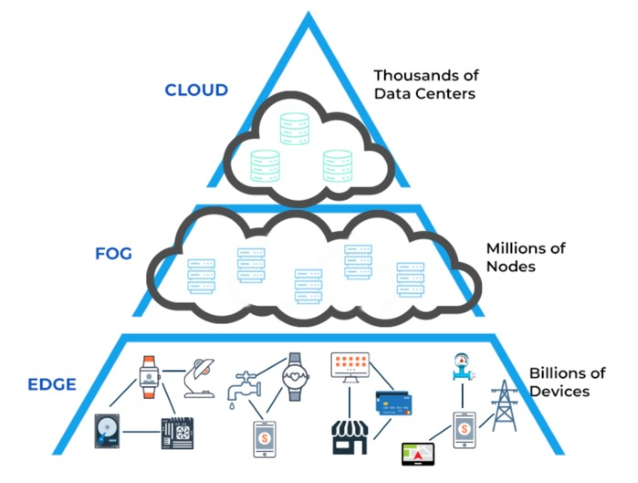
\includegraphics[width=\columnwidth]{images/EdgeArchitecture}	
	\caption{Edge Compute Architecture}
	\label{fig:EdgeArchitecture}
\end{figure}


According to research by IoT Analytics, there were 14.4 smart devices connected to the internet in 2022, expected to rise to almost 30 million by 2025\cite{IoTMarket}.  This many deployed devices could not be supported if they required connectivity to the large cloud data centers discussed earlier. Processing will need to move to the devices themselves supported by a new layer of cloud compute that is closer to the devices.  This new layer of compute is often referred to as \textit{fog computing}.  The term comes from a play on the word cloud, given clouds are high up in the sky and fog is closer to the ground.   


As cloud providers expand their footprint across the globe, creating new regions with multiple availability zones represents an expensive and time consuming investment. Creating new regions is required to increase compute capacity as global cloud adoption expands, and to meet specific compliance requirements associated with conducting business in the cloud. For example, many countries are adopting data residency laws, which place controls over where data is stored at rest. 

In many cases, new regions are not required, but cloud applications continue to push for better performance, which in many cases needs to be achieved via providing lower latency.  Approaches to lower latency have been deployed before the modern cloud with content delivery network (CDN)\cite{CDN} solutions.

\section{The Expansion of Software Engineering Concerns}
\label{sec:Polyglot}
The evolution of cloud computing over the past decade has increased the decision landscape for software engineers. This section will highlight some of the new concerns that software engineers must address in cloud and edge computing designs.

\subsection{Hardware and Processor Diversity}
Ten years ago we did not have cloud providers creating custom processors for compute, special purpose AI applications, nor did we have all of the microcontrollers running at the edge of the internet. Familiarity with making informed hardware architecture choices now becomes an important concern of software engineers. Some examples include:

\begin{itemize}
	\item On May 23, 2023, AWS announced the third generation of their custom ARM-based microprocessor called Graviton 3.  AWS Claims that workloads running on Graviton 3 are 50\% faster than Intel/AMD processors, consumer 60\% less power, and are 20\% cheaper. From a software engineering perspective these benefits seem like a no brainer to take advantage of until you start to factor in other requirements such as being able to maintain ARM-based builds of your software, including all dependencies. 
		
	\item Since the realization that GPUs can improve the performance of training AI models, cloud providers have innovated further with custom AI microprocessors.  In 2016 Google introduced the Tensor Processing Unit (TPU) to accelerate deep learning models, and in 2018 AWS created the Inferentia chip to accelerate inference. AWS also entered the training space to compete with Google's TPU with the Trainium chip in 2020.  With all of these new AI hardware choices, software engineers must be savvy with aligning hardware choices with software training libraries. For example, AWS announced a SDK for Trainium called Neuron to enable engineers to use popular libraries such as Tensorflow and PyTorch.  
	
	\item As we move to the edge, software engineers now more routinely have to create solutions for microcontollers, and other devices that have additional constraints.  These devices might be battery powered, compute constrained, difficult to access or update, and/or have unreliable network connectivity. Programming frameworks and tools routinely available on modern servers might not be available or viable for these devices.  Consider the popular trend of deploying code in containers.  To a large extent, containers make assumptions that there is an underlying linux kernel, which might not be possible in these purpose-built devices. Instead of falling back to creating alternative versions of their software in lower level systems programming languages like C/C++, software engineers must become familiar with emerging solutions in this space.  Consider TinyGo\cite{TinyGo}, which is an alternative Go compiler specifically created to bring the Go ecosystem, which is popular in the cloud, to microcontrollers.  Another example, is WasmEdge\cite{WASMEdge}, which brings the power of Web Assembly(WASM) to the server and to edge devices.  WasmEdge can run embedded WASM code created by modern compilers that are popular for creating cloud native applications such as Rust, Go, and Javascript.       
	
	\item Managing tool chains for multiple hardware architectures.  The Java programming language introduced the concept of \textit{"Write Once, Run Anywhere"}. It accomplished this by creating Java Virtual Machines (JVMs) for different hardware platforms, and running compiled bytecode consistently across these platforms.  While this works well, the Java ecosystem has some challenges in the broader cloud native space.  Specifically, to use Java all dependencies must be Java-based, and although the JVM itself is an impressive, its size and compute requirements might be challenging to support on edge devices. Newer programming languages like Rust and Go have been adopting an open cross-compiler philosophy so that any compiler on any platform can create binaries for any other platform.  Containers are another popular cloud native technology.  With the need to support diverse processor architectures container packaging becomes more complex, and containers might not be practical on the edge given they assume the presence of a linux kernel.  Docker recently released a technical preview to support web assembly that may help address this issue\cite{DockerWASM}.
\end{itemize}
 
\subsection{Polyglot Programming}
We think the move to cloud native architectures requires software engineers to rethink the criteria for how programming languages are selected.  In 2013 Meyerovich and Rabkin\cite{meyerovich2013empirical} reported on empirical human factors that impact programming language selection.  Their findings cite reasons such as open source libraries, existing code, and programmer experience as the primary drivers for selecting programming languages for new projects. To complicate matters further, in some organizations approved programming languages are standardized removing the software engineering community from the decision making loop.

The general criteria to evaluate programming languages often examines attributes like object-oriented vs functional; high-level vs low-level; type safety vs dynamic; general purpose or domain specific, and so on.  While these are good attributes to categorize programming languages they don't factor in criteria aligned to cloud native computing objectives.  For example\cite{flauzino2018you} did a comparative analysis of Java vs Kotlin.  Kotlin has been increasing in popularity within the Java community because it is less verbose, introduces modern programming language features, while interoperating well with existing Java code.  One of the criteria for good cloud native software discussed earlier is being able to move fast, thus adopting a language like Kotlin that is more productive and easier to test represents a good engineering tradeoff for organizations with significant investments and skillsets in Java. 

We think an approach for programming language selection should be based on a careful tradeoff analysis using cloud native computing architecture decisions to guide the selection.  This will often lead to a polyglot outcome, where more than one programming language is selected.  One interesting study in this space was conducted by Cordingly et. al.\cite{Serverless} where they examined the Java, Python, Go, and Node.js against a collection of different Function as a Service (FaaS) workloads.  We like their strategy using drivers such as performance and cost as the evaluation criteria.  They also used specific FaaS concerns such as cold and warm start times in their analysis. 

We think the approach used by Cordingly should be expanded to other cloud native architecture options.  For example, with container based solutions, languages like Java tend to produce very large containers, and require significant resources associated with bringing along the JVM.  Modern languages like Go, designed with the cloud in mind\footnote{Go is the primary language used to build significant cloud native platforms like Docker and Kubernetes}, produce very small containers, and has a robust and modern runtime.  Languages like Javascript and Typescript coupled with the Node.js runtime is highly optimized to support asynchronous event-based architectures. Languages like Rust provide C/C++ performance, but have a modern runtime and provide compiler-enforced memory safety. In addition to the languages themselves, additional factors such as the maturity and completeness of cloud provider supplied SDKs should also be considered in the selection criteria. 

\subsection{Multi-Cloud}
The major cloud providers run massive infrastructures that have historically have provided availability data that any individual enterprise would envy. However, while rare, cloud providers have had outages that have resulted in significant impact to customers. As cloud adoption continues to grow, the impact of these periodic outages will also continue to grow.  Additionally, the major cloud providers compete with each other via their innovation investments into fully managed services.  This has consequences of cloud vendor lock-in, making it hard for a customer to migrate from one cloud provider to another based on having to redevelop software 

\begin{itemize}
	\item Moving from Single to Multi-Region
	\item Diversifying services across multiple cloud providers
	\item Being able to be multi-cloud, running 
\end{itemize}  

\section{Cloud Computing Education}


\section{Conclusion}


\section{Acknowledgements}
We would like to thank the following individuals for their valuable feedback to this paper. 

\bibliography{CloudNative.bib}
\end{document} 